\documentclass[conference]{IEEEtran}
\usepackage[utf8]{inputenc}
\usepackage[portuguese]{babel}
\usepackage{amsmath}
\usepackage{algorithm}
\usepackage{algorithmic}
\usepackage{graphicx}
\usepackage{cite}
\usepackage{url}
\usepackage{enumitem}
\usepackage{booktabs}
\usepackage{multirow}
\usepackage{float}

\setlist[itemize]{itemsep=3pt, parsep=3pt, topsep=3pt}

\graphicspath{{graficos/}}

\begin{document}

\title{Análise Comparativa de Algoritmos de Ordenação em Estruturas de Dados Dinâmicas e Estáticas}

\author{
\IEEEauthorblockN{Elder Rayan Oliveira Silva, Samuel Wagner Tiburi Silveira, Diogo Gomes Figueiredo, \\
Manoel Junio Duarte da Silva, Pedro Yan Alcantara Palácio, Antonio Pereira da Luz Neto}
\IEEEauthorblockA{
Universidade Federal do Cariri -- UFCA\\
Engenharia de Software\\
Disciplina: Estrutura de Dados\\
}
}

\maketitle

% ============================================================
\begin{abstract}
Este trabalho apresenta uma análise comparativa do desempenho de cinco algoritmos clássicos de ordenação --- Bubble Sort, Selection Sort, Insertion Sort, Quick Sort e Merge Sort --- aplicados a três estruturas de dados distintas: vetor convencional, lista duplamente encadeada dinâmica e lista duplamente encadeada estática. A aplicação real escolhida foi um sistema de ranking de alunos, no qual registros contendo identificador e nota são ordenados de forma crescente. Os experimentos foram conduzidos na linguagem C, com 100 execuções por cenário, variando o volume de dados (100, 1.000 e 10.000 elementos) e o tipo de entrada (aleatório, ordenado e inversamente ordenado). Os resultados confirmam a superioridade assintótica dos algoritmos $O(n \log n)$: o Merge Sort apresentou os menores tempos médios em praticamente todos os cenários, com tempo de 1,36\,ms para 10.000 elementos aleatórios em vetor, enquanto o Bubble Sort registrou 142,05\,ms na mesma configuração. A análise do impacto da estrutura de dados revelou que o vetor convencional oferece o melhor desempenho geral, seguido pela lista dinâmica, sendo a lista estática a mais lenta devido ao custo de navegação por índices. O Merge Sort foi selecionado como algoritmo ideal para a aplicação proposta, dada sua garantia de desempenho $O(n \log n)$ em todos os casos e sua propriedade de estabilidade.
\end{abstract}

\begin{IEEEkeywords}
Algoritmos de ordenação, estruturas de dados, lista encadeada, análise de desempenho, complexidade computacional.
\end{IEEEkeywords}

% ============================================================
\section{Introdução}
% ============================================================

A escolha adequada de algoritmos de ordenação e estruturas de dados é um problema fundamental em Ciência da Computação, com impacto direto no desempenho de sistemas reais~\cite{cormen,sedgewick}. Em aplicações que manipulam grandes volumes de dados --- como sistemas de ranking acadêmico, plataformas de \textit{e-commerce} e aplicativos de entrega --- a eficiência da ordenação pode determinar a viabilidade do sistema sob restrições de tempo de resposta.

Embora a análise teórica de complexidade assintótica forneça uma estimativa do comportamento dos algoritmos, fatores práticos como localidade de cache, overhead de alocação de memória e a estrutura de dados subjacente influenciam significativamente o desempenho real~\cite{knuth,ziviani}. Assim, a avaliação empírica complementa a análise teórica e permite decisões de projeto mais informadas.

Este trabalho tem como objetivo analisar o impacto da escolha de estruturas de dados e algoritmos de ordenação no desempenho de uma aplicação real de ranking de alunos. Para isso, foram implementados cinco algoritmos clássicos de ordenação (Bubble Sort, Selection Sort, Insertion Sort, Quick Sort e Merge Sort) sobre três estruturas de dados (vetor, lista duplamente encadeada dinâmica e lista duplamente encadeada estática), com avaliação empírica em diferentes volumes e padrões de entrada.

% ============================================================
\section{Fundamentação Teórica}
% ============================================================

\subsection{Estruturas de Dados Utilizadas}

Para avaliar o impacto da organização da memória no desempenho dos algoritmos, foram implementadas três estruturas de dados para armazenar registros de alunos (identificador e nota):

\subsubsection{Vetor Convencional}
Estrutura contígua em memória com acesso direto por índice em $O(1)$. Oferece a melhor localidade de cache, mas possui tamanho fixo.

\subsubsection{Lista Duplamente Encadeada Dinâmica}
Utiliza alocação de memória sob demanda via \texttt{malloc()} e \texttt{free()}. Cada nó armazena identificador, nota e ponteiros para o nó anterior e o próximo. Oferece flexibilidade de tamanho, mas sofre com fragmentação de memória e localidade de cache prejudicada.

\subsubsection{Lista Duplamente Encadeada Estática}
Simula uma lista duplamente encadeada utilizando um vetor pré-alocado, onde os ``ponteiros'' são índices inteiros. Uma lista auxiliar de posições livres gerencia a reutilização de espaços. Combina contiguidade de memória com a lógica de encadeamento, mas adiciona complexidade no gerenciamento de índices.

\subsection{Algoritmos de Ordenação}

\subsubsection{Bubble Sort}
Algoritmo baseado em comparações sucessivas de elementos adjacentes. Apresenta complexidade $O(n)$ no melhor caso (lista já ordenada, com otimização de \textit{flag}) e $O(n^2)$ nos casos médio e pior. É in-place e estável~\cite{cormen,sedgewick}.

\subsubsection{Selection Sort}
Seleciona o menor elemento não ordenado a cada iteração. Apresenta complexidade $O(n^2)$ em todos os casos, pois sempre percorre os elementos restantes. É in-place, porém não estável na implementação padrão~\cite{cormen}.

\subsubsection{Insertion Sort}
Insere cada elemento na posição correta da porção já ordenada. Apresenta complexidade $O(n)$ no melhor caso e $O(n^2)$ nos demais. É adaptativo: para uma lista com $k$ inversões, opera em $O(n + k)$. In-place e estável~\cite{cormen,knuth}.

\subsubsection{Quick Sort}
Algoritmo de divisão e conquista que particiona o vetor em torno de um pivô. Apresenta complexidade $O(n \log n)$ nos casos melhor e médio, mas pode degradar para $O(n^2)$ no pior caso (pivô extremo). Utiliza memória $O(\log n)$ para a pilha de recursão. É in-place, porém não estável~\cite{sedgewick,knuth}.

\subsubsection{Merge Sort}
Divide recursivamente a estrutura em metades, ordena cada uma e as intercala. Apresenta complexidade $O(n \log n)$ em todos os casos --- melhor, médio e pior. Para o vetor, utiliza memória auxiliar $O(n)$. É estável e previsível~\cite{cormen,knuth}.

\subsection{Tabela Comparativa de Complexidade}

A Tabela~\ref{tab:complexidade} resume a complexidade teórica dos cinco algoritmos.

\begin{table}[htbp]
\centering
\caption{Complexidade de tempo e espaço dos algoritmos}
\label{tab:complexidade}
\renewcommand{\arraystretch}{1.3}
\begin{tabular}{lcccl}
\toprule
\textbf{Algoritmo} & \textbf{Melhor} & \textbf{Médio} & \textbf{Pior} & \textbf{Espaço} \\
\midrule
Bubble Sort    & $O(n)$       & $O(n^2)$      & $O(n^2)$      & $O(1)$ \\
Selection Sort & $O(n^2)$     & $O(n^2)$      & $O(n^2)$      & $O(1)$ \\
Insertion Sort & $O(n)$       & $O(n^2)$      & $O(n^2)$      & $O(1)$ \\
Quick Sort     & $O(n \log n)$& $O(n \log n)$ & $O(n^2)$      & $O(\log n)$ \\
Merge Sort     & $O(n \log n)$& $O(n \log n)$ & $O(n \log n)$ & $O(n)$ \\
\bottomrule
\end{tabular}
\end{table}

% ============================================================
\section{Metodologia}
% ============================================================

\subsection{Aplicação Real: Sistema de Ranking de Alunos}

O cenário escolhido simula um sistema de ranking acadêmico no qual registros de alunos (contendo identificador e nota de 0 a 100) são ordenados por nota de forma crescente. Esse cenário é representativo de aplicações reais onde listas precisam ser ordenadas dinamicamente conforme novos registros são inseridos ou removidos.

\subsection{Ambiente de Desenvolvimento e Testes}

A implementação foi realizada na linguagem C, compilada com GCC (MinGW) 8.1.0 em ambiente Windows. Os gráficos de análise foram gerados em Python~3.11 utilizando as bibliotecas \texttt{pandas}, \texttt{matplotlib} e \texttt{seaborn}. O código-fonte foi organizado em módulos separados para algoritmos, estruturas de dados e utilitários de medição.

\subsection{Variáveis de Teste}

Os experimentos foram conduzidos variando três dimensões:

\begin{itemize}
    \item \textbf{Volume de dados ($N$):} 100 (pequeno), 1.000 (médio) e 10.000 (grande) elementos.
    \item \textbf{Tipo de entrada:} Aleatório (caso médio), Ordenado (melhor caso para algoritmos adaptativos) e Inversamente Ordenado (pior caso).
    \item \textbf{Estrutura de dados:} Vetor convencional, Lista Dinâmica e Lista Estática.
\end{itemize}

\subsection{Protocolo de Medição}

Cada combinação de algoritmo, estrutura, tamanho e tipo de entrada foi executada 100 vezes. O tempo de execução foi medido utilizando a função \texttt{clock()} da biblioteca padrão C, cronometrando exclusivamente o trecho de ordenação, sem incluir geração de dados ou operações de entrada/saída. A métrica principal é a média dos tempos em milissegundos.

% ============================================================
\section{Implementação}
% ============================================================

\subsection{Estruturas de Dados}

Cada registro de aluno é representado pela estrutura \texttt{Aluno}, contendo campos inteiro \texttt{id} e ponto flutuante \texttt{nota}. As operações fundamentais (inicialização, inserção, busca, remoção e liberação) foram implementadas para ambas as listas encadeadas.

Na \textbf{lista dinâmica}, cada nó é alocado individualmente via \texttt{malloc()}, com ponteiros \texttt{prox} e \texttt{ant}. Na \textbf{lista estática}, os nós residem em um vetor pré-alocado de tamanho fixo, com ``ponteiros'' representados por índices inteiros e uma lista de posições livres.

\subsection{Algoritmos de Ordenação}

Cada algoritmo foi implementado em três versões: uma para vetor, uma para lista dinâmica e uma para lista estática. As adaptações principais são:

\begin{itemize}
    \item \textbf{Vetor:} acesso direto por índice; trocas via variável temporária do tipo \texttt{Aluno}.
    \item \textbf{Lista Dinâmica:} navegação por ponteiros; trocas de dados entre nós (sem remanejamento de ponteiros, exceto no Merge Sort).
    \item \textbf{Lista Estática:} navegação por índices no vetor; trocas de campos \texttt{id} e \texttt{nota} entre posições.
\end{itemize}

O \textbf{Bubble Sort} utiliza uma \textit{flag} de troca para encerrar antecipadamente quando a estrutura já está ordenada. O \textbf{Quick Sort} emprega a estratégia de pivô no último elemento com otimização \textit{tail-call} (recursa no menor lado e itera no maior), reduzindo a profundidade máxima da pilha. O \textbf{Merge Sort} no vetor aloca um array temporário de tamanho $n$; nas listas encadeadas, a intercalação é realizada por religação de ponteiros/índices sem alocação extra significativa.

\subsection{Algoritmo Ideal: Merge Sort}

O Merge Sort foi selecionado como algoritmo ideal para a aplicação de ranking, pelas seguintes razões:

\begin{enumerate}
    \item \textbf{Garantia de desempenho:} complexidade $O(n \log n)$ em todos os casos, sem risco de degradação para $O(n^2)$.
    \item \textbf{Estabilidade:} preserva a ordem relativa de alunos com mesma nota, permitindo ordenações compostas (por nota e depois por nome, por exemplo).
    \item \textbf{Previsibilidade:} essencial em sistemas críticos onde o tempo de resposta deve ser garantido.
\end{enumerate}

O funcionamento segue o paradigma de divisão e conquista em três fases:

\begin{algorithmic}
\IF{$n \leq 1$}
    \RETURN
\ENDIF
\STATE $meio \gets n / 2$
\STATE Divide estrutura em metade esquerda $L$ e metade direita $R$
\STATE MergeSort($L$)
\STATE MergeSort($R$)
\STATE Intercala $L$ e $R$ em ordem crescente
\end{algorithmic}

O custo espacial $O(n)$ é o principal \textit{trade-off}, porém aceitável em sistemas modernos com memória abundante.

% ============================================================
\section{Resultados e Análise}
% ============================================================

Esta seção apresenta os resultados experimentais, organizados em análises progressivas: comparação geral, impacto do tipo de entrada, impacto da estrutura de dados e comportamento individual dos algoritmos.

\subsection{Comparação Geral de Desempenho}

A Figura~\ref{fig:grafico1} apresenta o tempo médio de cada algoritmo para $N=10.000$ com entrada aleatória (dados de vetor, caso médio). Nesse cenário específico, o Quick Sort apresenta o menor tempo (1,01\,ms), seguido pelo Merge Sort (1,36\,ms). Os algoritmos $O(n^2)$ são drasticamente mais lentos: Insertion Sort (40,14\,ms), Selection Sort (54,85\,ms) e Bubble Sort (142,05\,ms).

\begin{figure}[htbp]
    \centering
    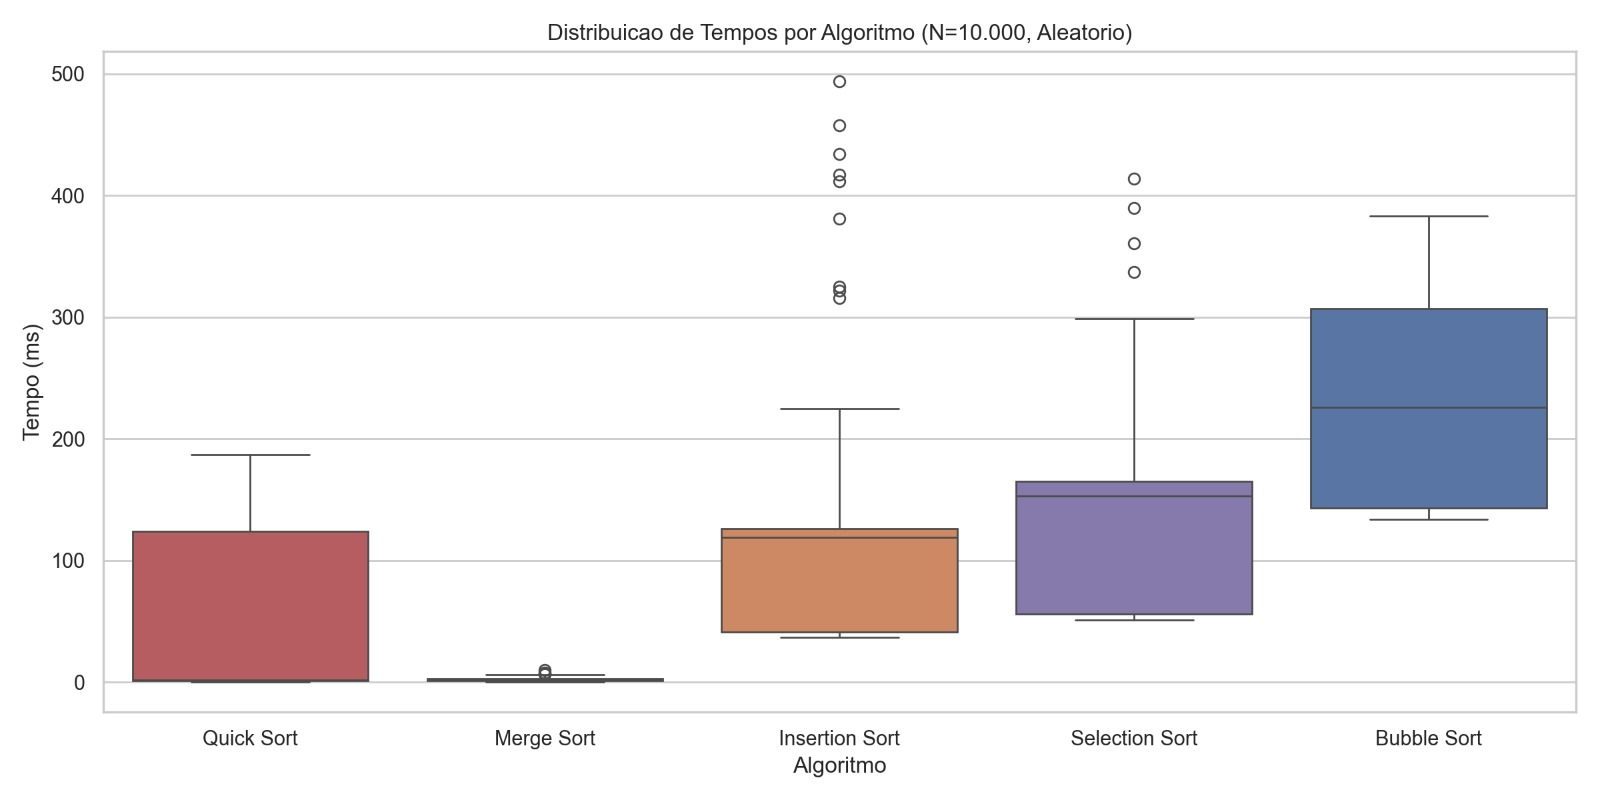
\includegraphics[width=\columnwidth]{grafico_1_comparacao_geral_10k.png}
    \caption{Comparação geral --- tempo médio por algoritmo ($N=10.000$, aleatório). O Merge Sort é quase imperceptível na escala; ver Figura~\ref{fig:grafico1zoom} para ampliação.}
    \label{fig:grafico1}
\end{figure}

\begin{figure}[htbp]
    \centering
    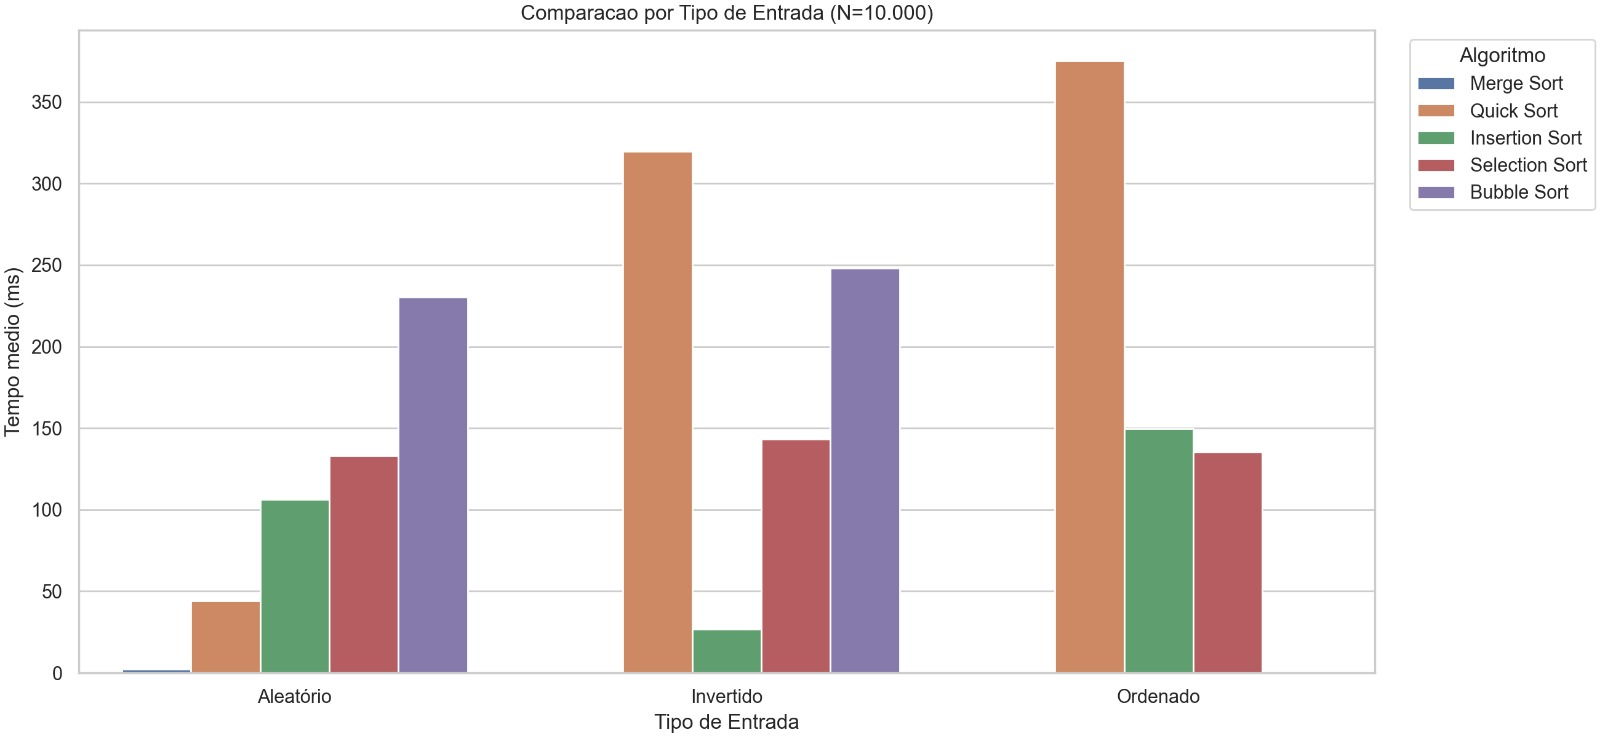
\includegraphics[width=\columnwidth]{grafico_1_comparacao_geral_10k_zoom.png}
    \caption{Ampliação da faixa de tempos até 10\,ms. O Merge Sort (1,36\,ms) e o Quick Sort (1,01\,ms em vetor) ficam claramente visíveis.}
    \label{fig:grafico1zoom}
\end{figure}

A diferença de duas ordens de grandeza entre os grupos $O(n^2)$ e $O(n \log n)$ confirma a análise teórica: para $N=10.000$, o fator $n^2 / (n \log n) \approx 750$, compatível com a razão observada $142{,}05 / 1{,}36 \approx 104$\footnote{A razão real é menor que a teórica pois as constantes multiplicativas dos algoritmos diferem.}.

\subsection{Curva de Crescimento}

A Figura~\ref{fig:grafico2} mostra a evolução do tempo médio em função de $N$ para entrada aleatória. Para $N=100$ e $N=1.000$, todos os algoritmos apresentam tempos próximos de zero. A separação se torna evidente a partir de $N=10.000$: enquanto Merge Sort e Quick Sort mantêm tempos abaixo de 2\,ms, o Bubble Sort ultrapassa 140\,ms, evidenciando o crescimento quadrático.

\begin{figure}[htbp]
    \centering
    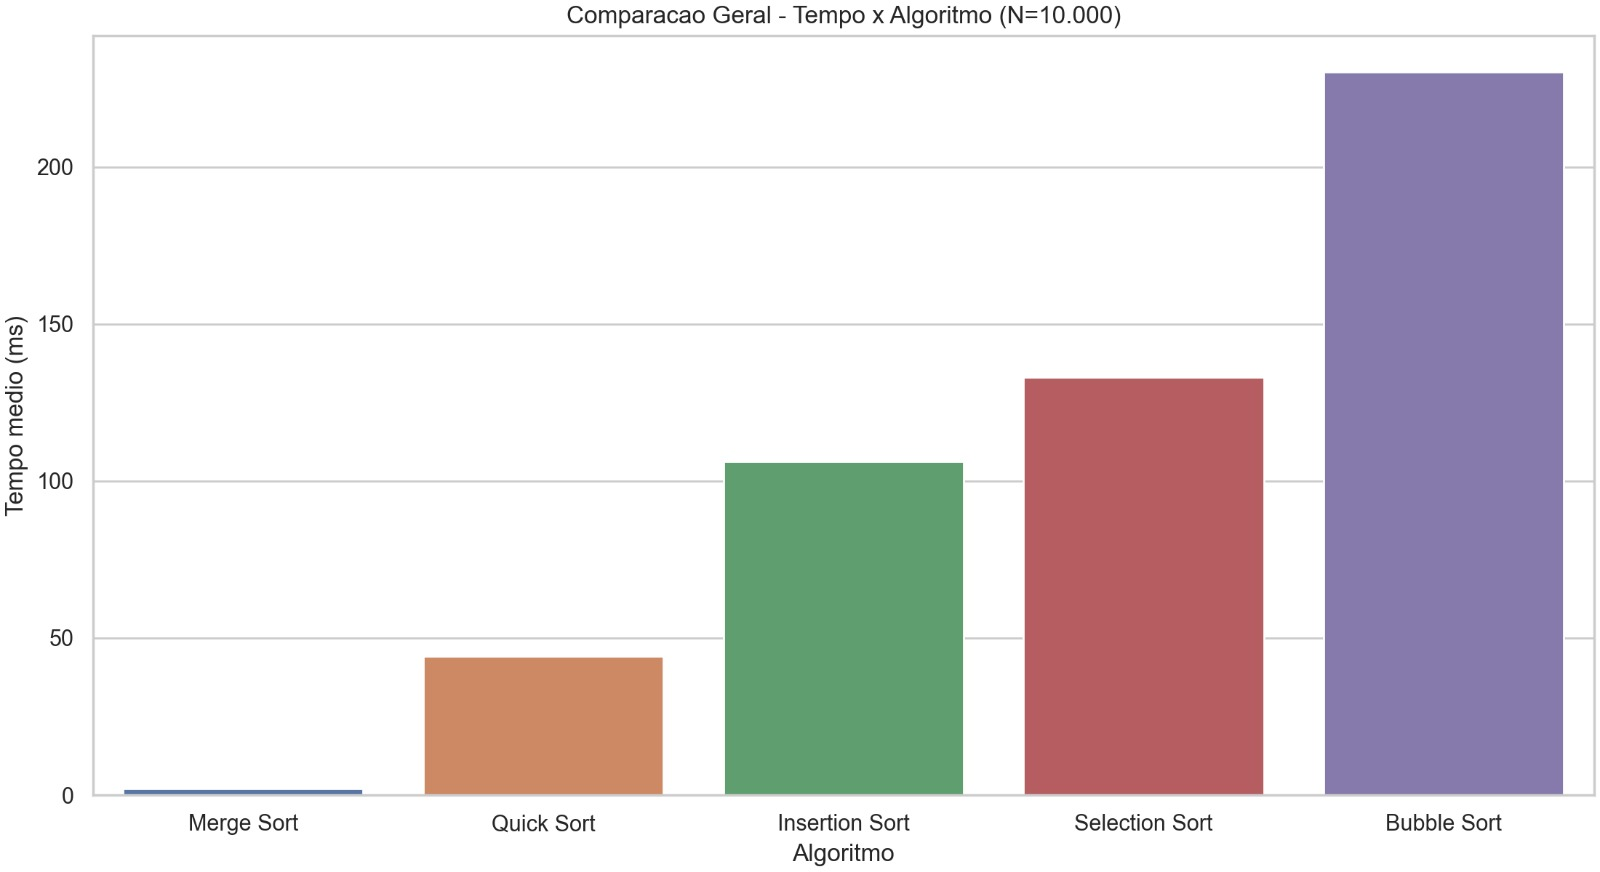
\includegraphics[width=\columnwidth]{grafico_2_curva_crescimento.png}
    \caption{Curva de crescimento --- tempo médio em função do tamanho do vetor (entrada aleatória).}
    \label{fig:grafico2}
\end{figure}

A curva do Merge Sort permanece praticamente plana na escala do gráfico, confirmando seu crescimento $O(n \log n)$. As curvas dos algoritmos quadráticos exibem o formato parabólico esperado.

\subsection{Impacto do Tipo de Entrada}

A Figura~\ref{fig:grafico4} apresenta o desempenho de cada algoritmo nos três tipos de entrada para $N=10.000$. Observam-se comportamentos notáveis:

\begin{figure}[htbp]
    \centering
    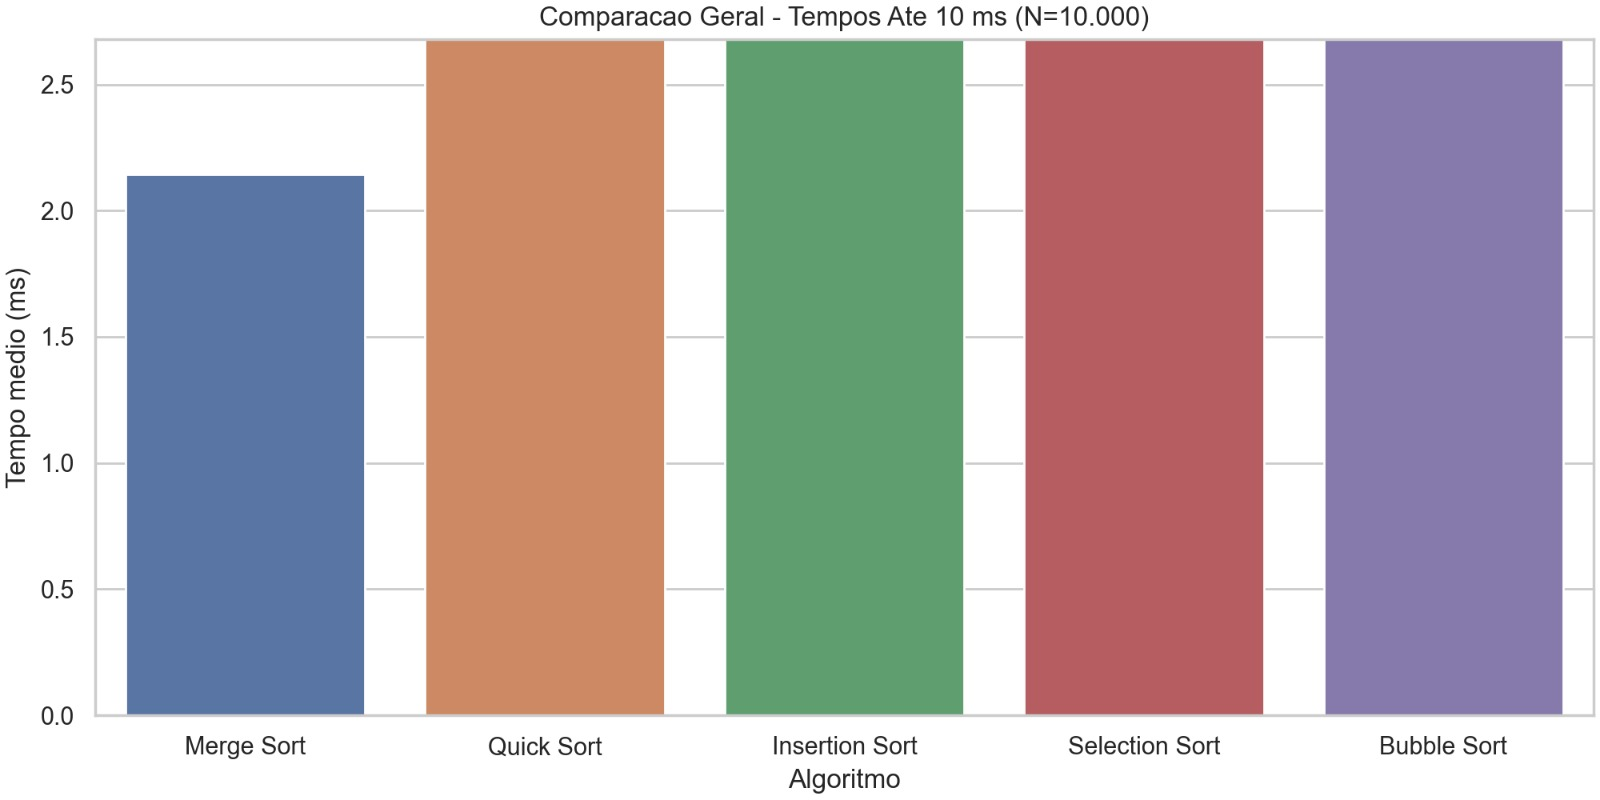
\includegraphics[width=\columnwidth]{grafico_4_por_tipo_entrada.png}
    \caption{Comparação por tipo de entrada ($N=10.000$). Merge Sort é quase imperceptível; ver Figura~\ref{fig:grafico4zoom}.}
    \label{fig:grafico4}
\end{figure}

\begin{figure}[htbp]
    \centering
    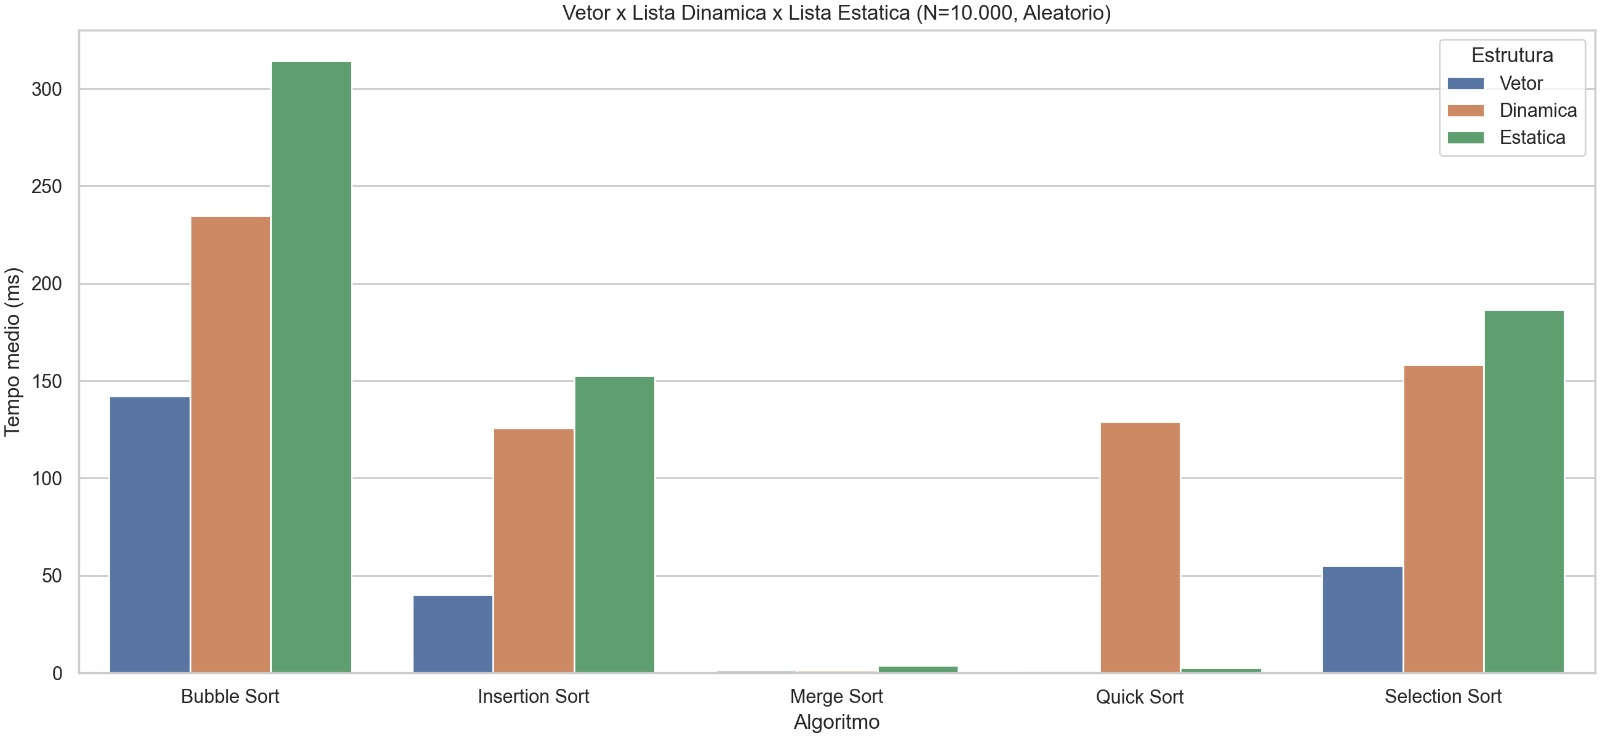
\includegraphics[width=\columnwidth]{grafico_4_por_tipo_entrada_zoom.png}
    \caption{Ampliação da faixa de tempos até 10\,ms para visualização do Merge Sort.}
    \label{fig:grafico4zoom}
\end{figure}

\begin{itemize}
    \item \textbf{Bubble Sort:} tempo próximo de zero para entrada ordenada (0,03\,ms), confirmando a otimização de \textit{flag}. Para entrada invertida, atinge 149,18\,ms.
    \item \textbf{Insertion Sort:} comportamento semelhante ao Bubble Sort --- 0,02\,ms para entrada ordenada e 80,12\,ms para invertida --- refletindo sua propriedade adaptativa.
    \item \textbf{Selection Sort:} tempos praticamente constantes ($\approx$54\,ms) independentemente do tipo de entrada, pois sempre percorre os $n-i$ elementos restantes.
    \item \textbf{Quick Sort:} degrada para entrada ordenada (138,91\,ms) e invertida (90,85\,ms) devido à escolha de pivô no último elemento, que gera partições desbalanceadas nesses cenários. Para dados aleatórios, opera em apenas 1,01\,ms.
    \item \textbf{Merge Sort:} desempenho consistente entre 0,50\,ms e 1,36\,ms em todos os cenários, confirmando sua complexidade $O(n \log n)$ invariante.
\end{itemize}

O Quick Sort, apesar de ser o mais rápido no caso aleatório (1,01\,ms), sofre degradação severa de até $138\times$ no caso ordenado. O Merge Sort mantém variação máxima de apenas $2{,}7\times$ entre seus extremos.

\subsection{Impacto da Estrutura de Dados}

A Figura~\ref{fig:grafico6} compara o desempenho das três estruturas para cada algoritmo ($N=10.000$, entrada aleatória).

\begin{figure}[htbp]
    \centering
    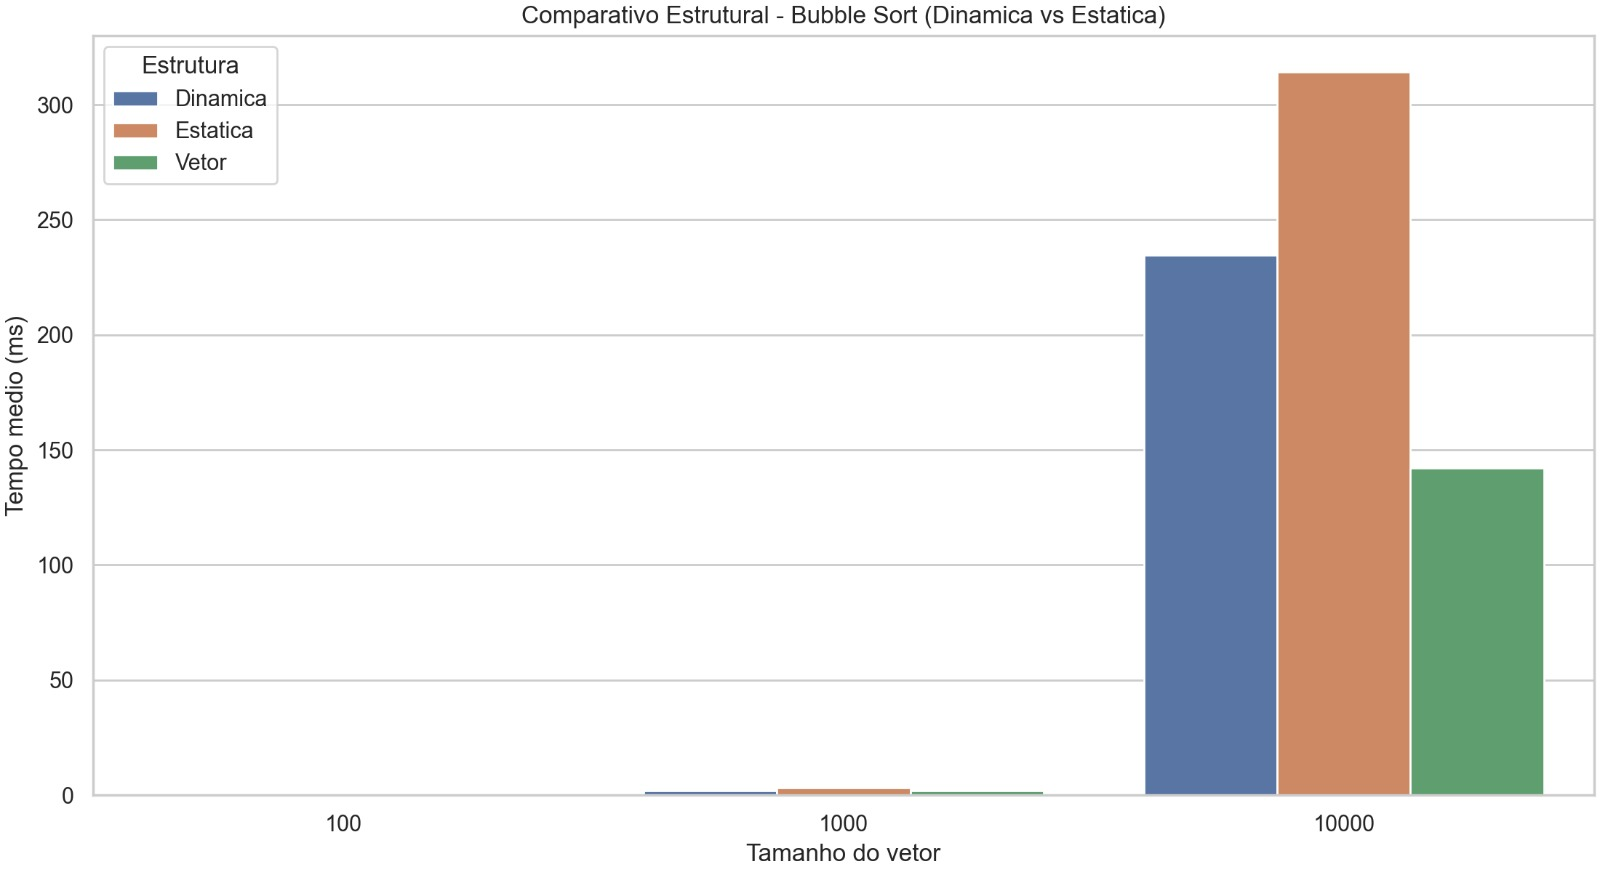
\includegraphics[width=\columnwidth]{grafico_6_vetor_x_dinamica_x_estatica.png}
    \caption{Comparação Vetor $\times$ Lista Dinâmica $\times$ Lista Estática ($N=10.000$, aleatório).}
    \label{fig:grafico6}
\end{figure}

\begin{figure}[htbp]
    \centering
    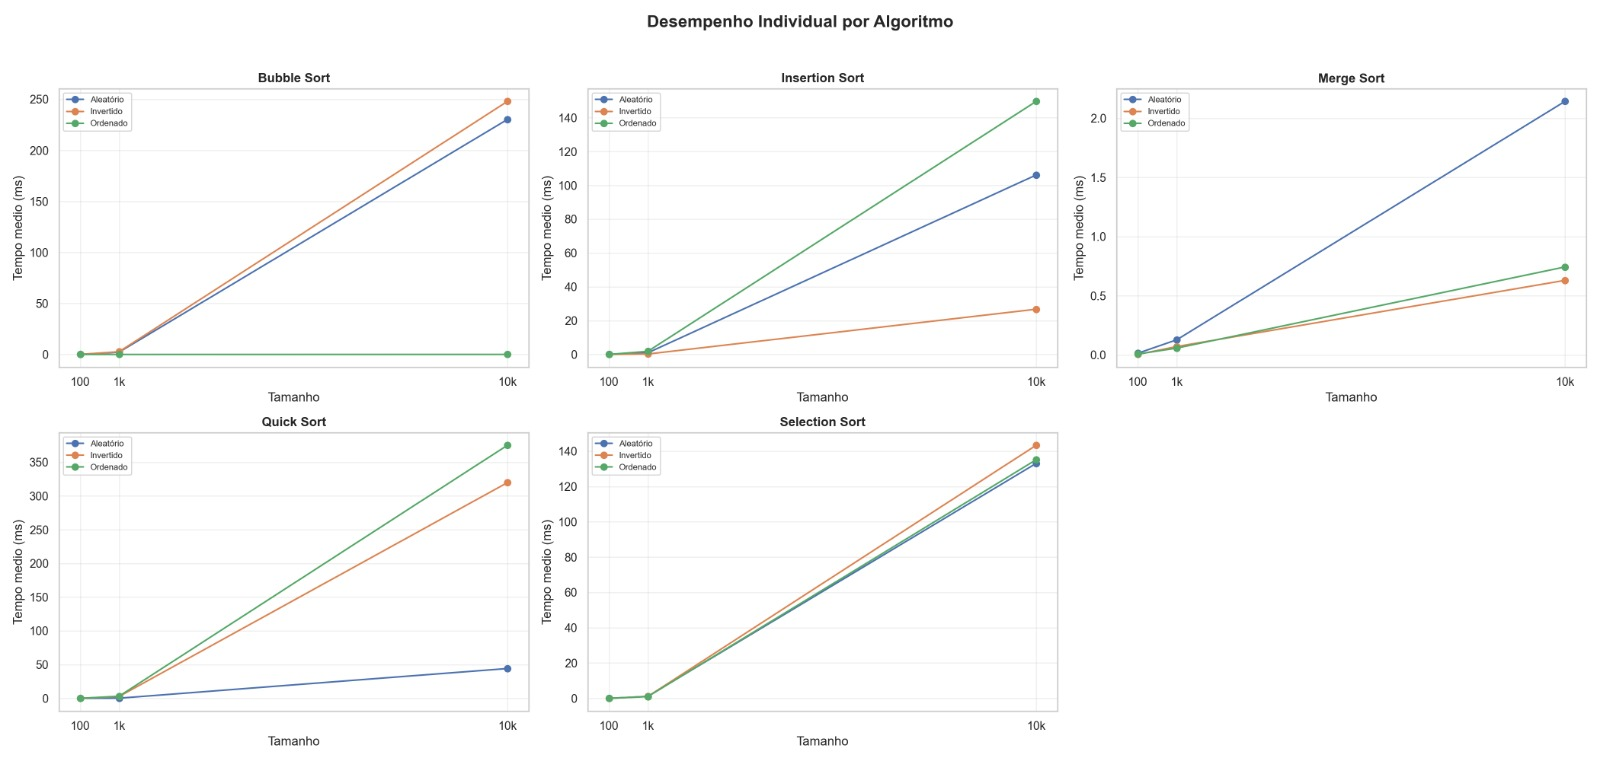
\includegraphics[width=\columnwidth]{grafico_6_vetor_x_dinamica_x_estatica_zoom.png}
    \caption{Ampliação da faixa até 10\,ms para o Merge Sort e Quick Sort.}
    \label{fig:grafico6zoom}
\end{figure}

Os dados revelam um padrão consistente: o \textbf{vetor} é a estrutura mais rápida, seguido pela \textbf{lista dinâmica} e pela \textbf{lista estática}. Para o Bubble Sort, por exemplo, os tempos foram 142,05\,ms (vetor), 234,55\,ms (dinâmica) e 314,27\,ms (estática) --- uma diferença de $2{,}2\times$ entre vetor e estática.

Este comportamento é explicado por dois fatores:
\begin{itemize}
    \item \textbf{Localidade de cache:} o vetor armazena elementos contiguamente, aproveitando ao máximo as linhas de cache da CPU. A lista dinâmica, com nós espalhados na \textit{heap}, provoca \textit{cache misses} frequentes.
    \item \textbf{Custo de navegação:} na lista estática, a navegação por índices (\texttt{l->dados[i].prox}) envolve indireção adicional em relação ao acesso direto do vetor, além de padrões de acesso não sequenciais que os prejudicam perante o pré-carregamento (\textit{prefetch}) da CPU.
\end{itemize}

\subsection{Comparativo Estrutural --- Bubble Sort}

A Figura~\ref{fig:grafico3} isolou o Bubble Sort para comparar as três estruturas em todos os tamanhos.

\begin{figure}[htbp]
    \centering
    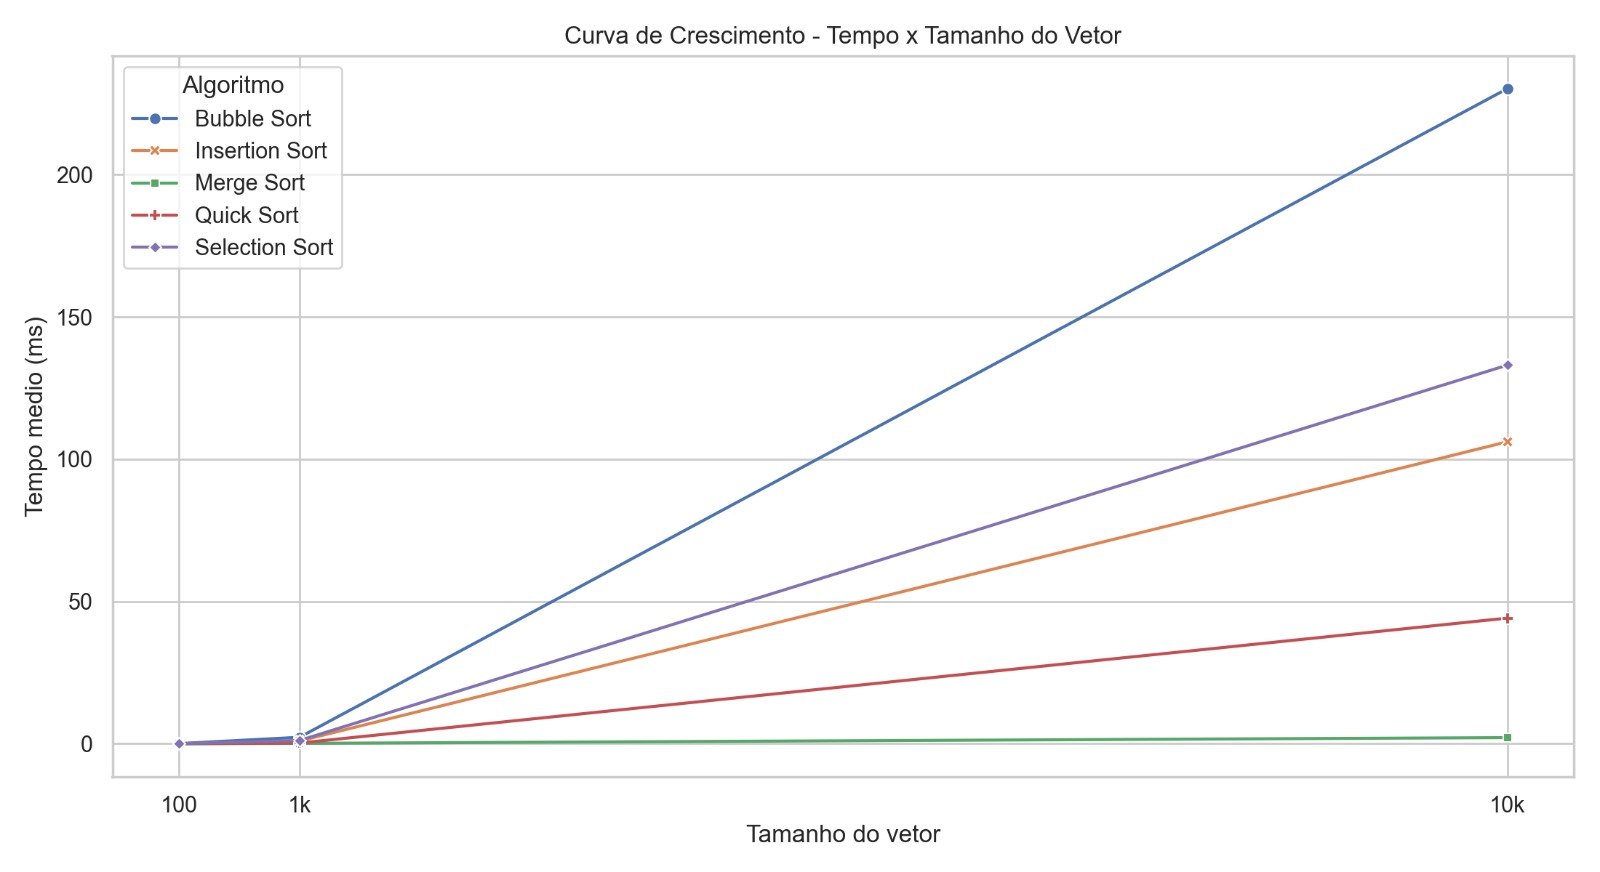
\includegraphics[width=\columnwidth]{grafico_3_comparativo_estrutural.png}
    \caption{Comparativo estrutural do Bubble Sort (Dinâmica $\times$ Estática $\times$ Vetor).}
    \label{fig:grafico3}
\end{figure}

Para $N=100$ e $N=1.000$, as diferenças são pequenas. Em $N=10.000$, a lista estática é aproximadamente $2{,}2\times$ mais lenta que o vetor, confirmando que o impacto da estrutura cresce com o volume de dados.

\subsection{Desempenho Individual por Algoritmo}

A Figura~\ref{fig:grafico5} apresenta o comportamento de cada algoritmo individualmente, mostrando tempo $\times$ tamanho $\times$ tipo de entrada.

\begin{figure}[htbp]
    \centering
    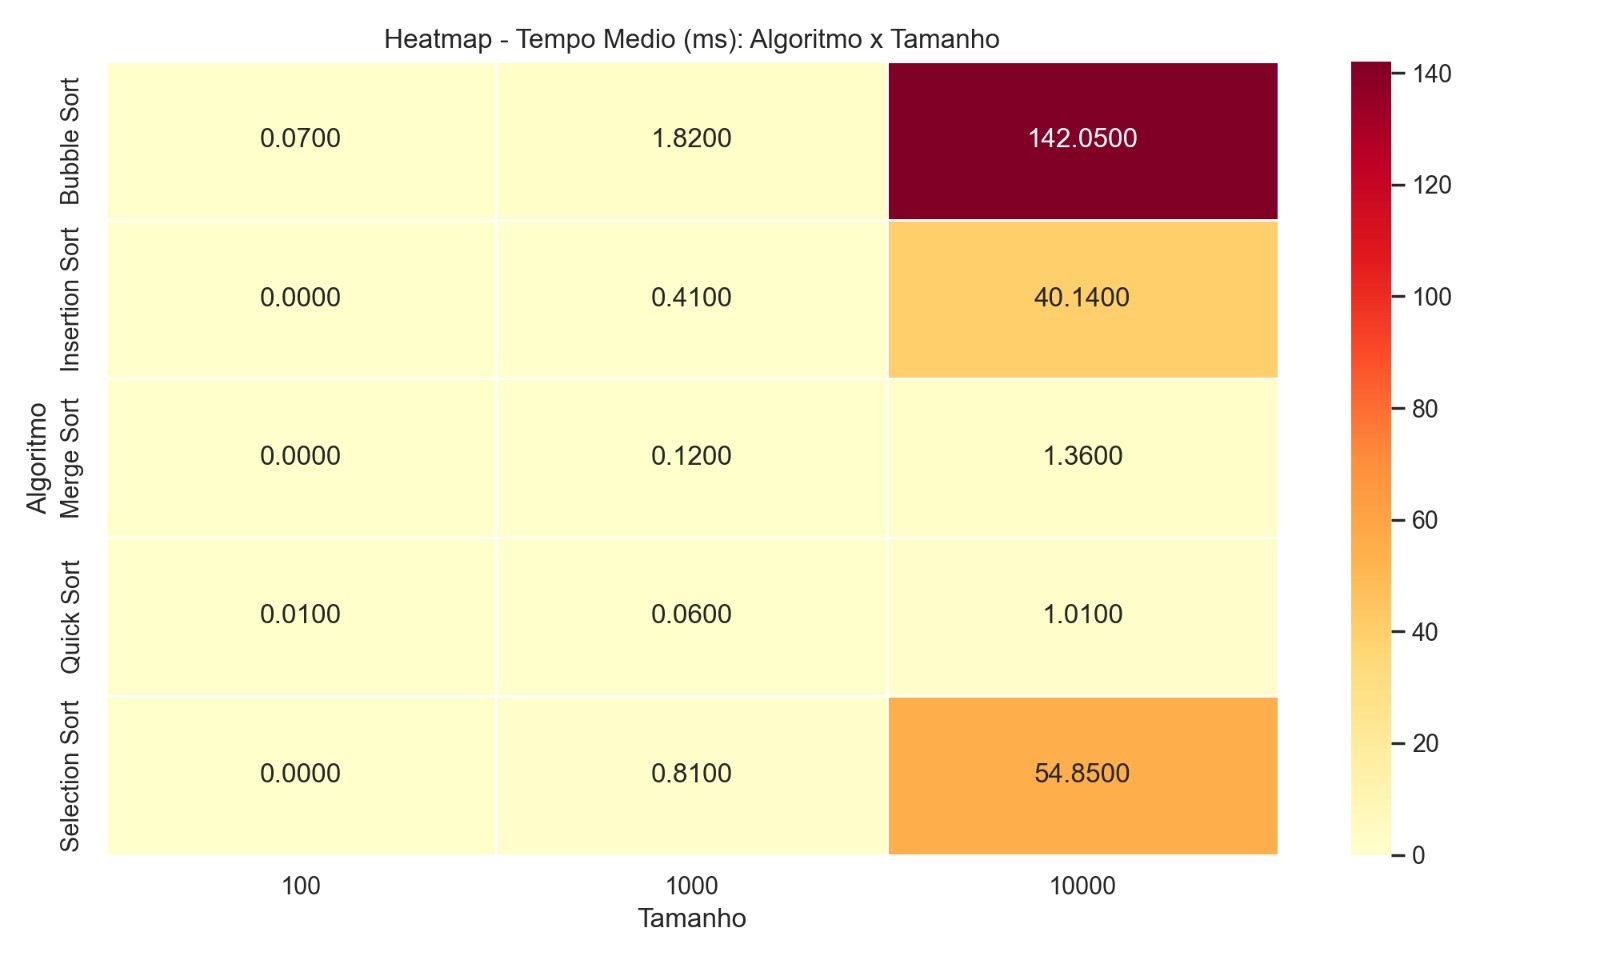
\includegraphics[width=\columnwidth]{grafico_5_por_algoritmo.png}
    \caption{Desempenho individual --- cada subplot mostra um algoritmo com curvas por tipo de entrada.}
    \label{fig:grafico5}
\end{figure}

Destaca-se o comportamento do \textbf{Quick Sort}, que inverte sua vantagem conforme o tipo de entrada: é o segundo mais rápido para dados aleatórios, mas o mais lento para dados ordenados e invertidos (devido ao pivô fixo no último elemento). O \textbf{Insertion Sort} apresenta padrão complementar: excelente para dados invertidos na lista dinâmica (0,04\,ms) e ordenados no vetor (0,02\,ms), graças à sua adaptatividade.

\subsection{Distribuição de Tempos}

A Figura~\ref{fig:grafico7} apresenta a dispersão dos tempos através de \textit{boxplots} para $N=10.000$.

\begin{figure}[htbp]
    \centering
    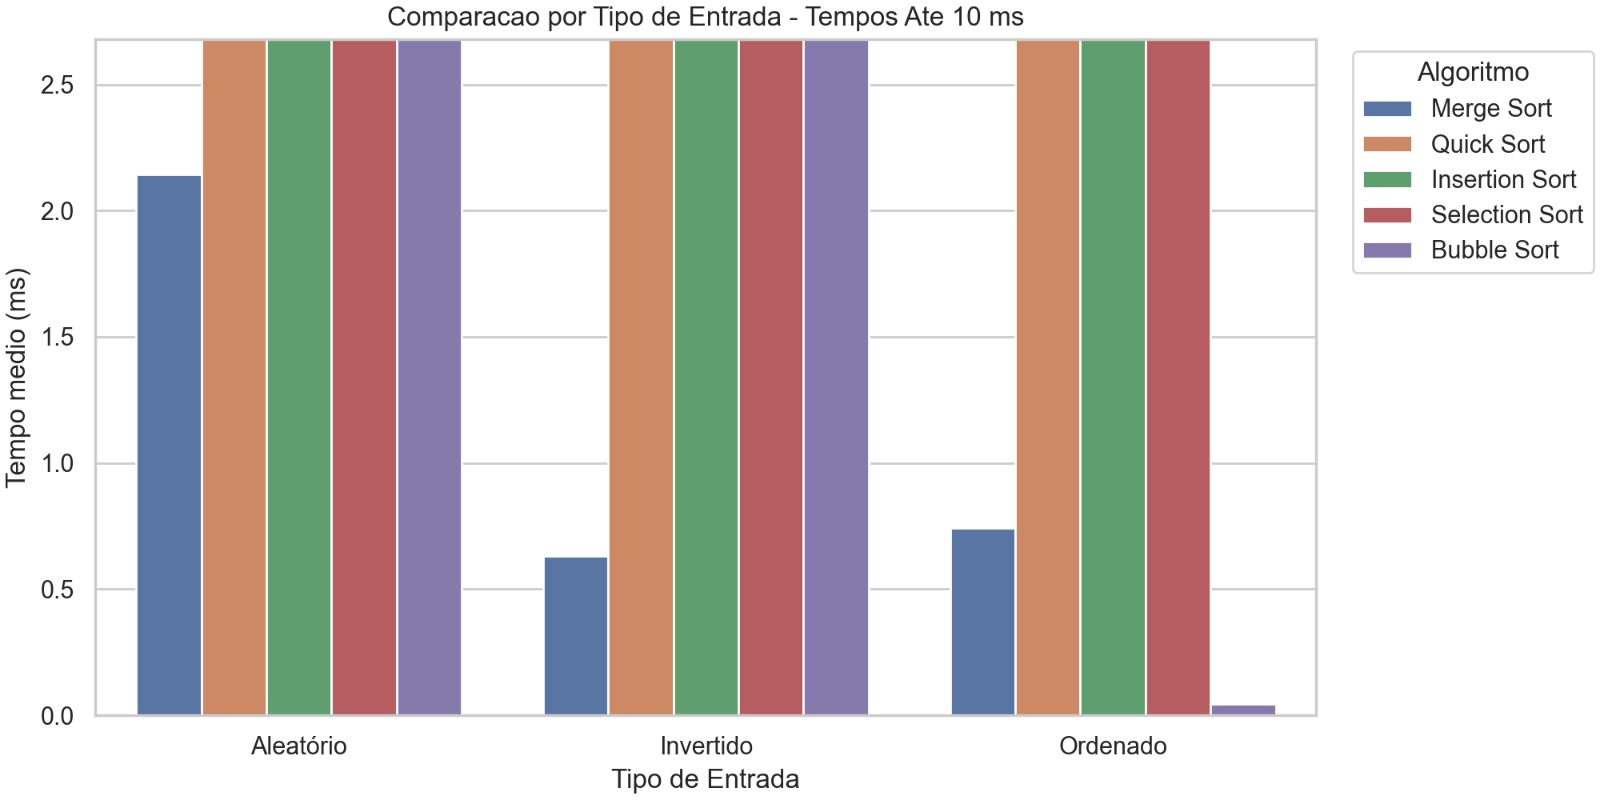
\includegraphics[width=\columnwidth]{grafico_7_boxplot_distribuicao.png}
    \caption{Distribuição de tempos por algoritmo ($N=10.000$). Os \textit{outliers} indicam variabilidade entre cenários.}
    \label{fig:grafico7}
\end{figure}

O Merge Sort concentra-se na faixa de 0 a 10\,ms com \textit{outliers} mínimos, demonstrando alta previsibilidade. O Quick Sort apresenta a maior dispersão, com mediana próxima de zero (caso do vetor com entrada aleatória) mas \textit{outliers} acima de 180\,ms (lista dinâmica com dados ordenados/invertidos).

\subsection{Heatmap e Ranking}

A Figura~\ref{fig:grafico8} apresenta o heatmap de tempos médios por algoritmo e tamanho (vetor, aleatório), e a Figura~\ref{fig:grafico9} mostra o ranking médio por cenário.

\begin{figure}[htbp]
    \centering
    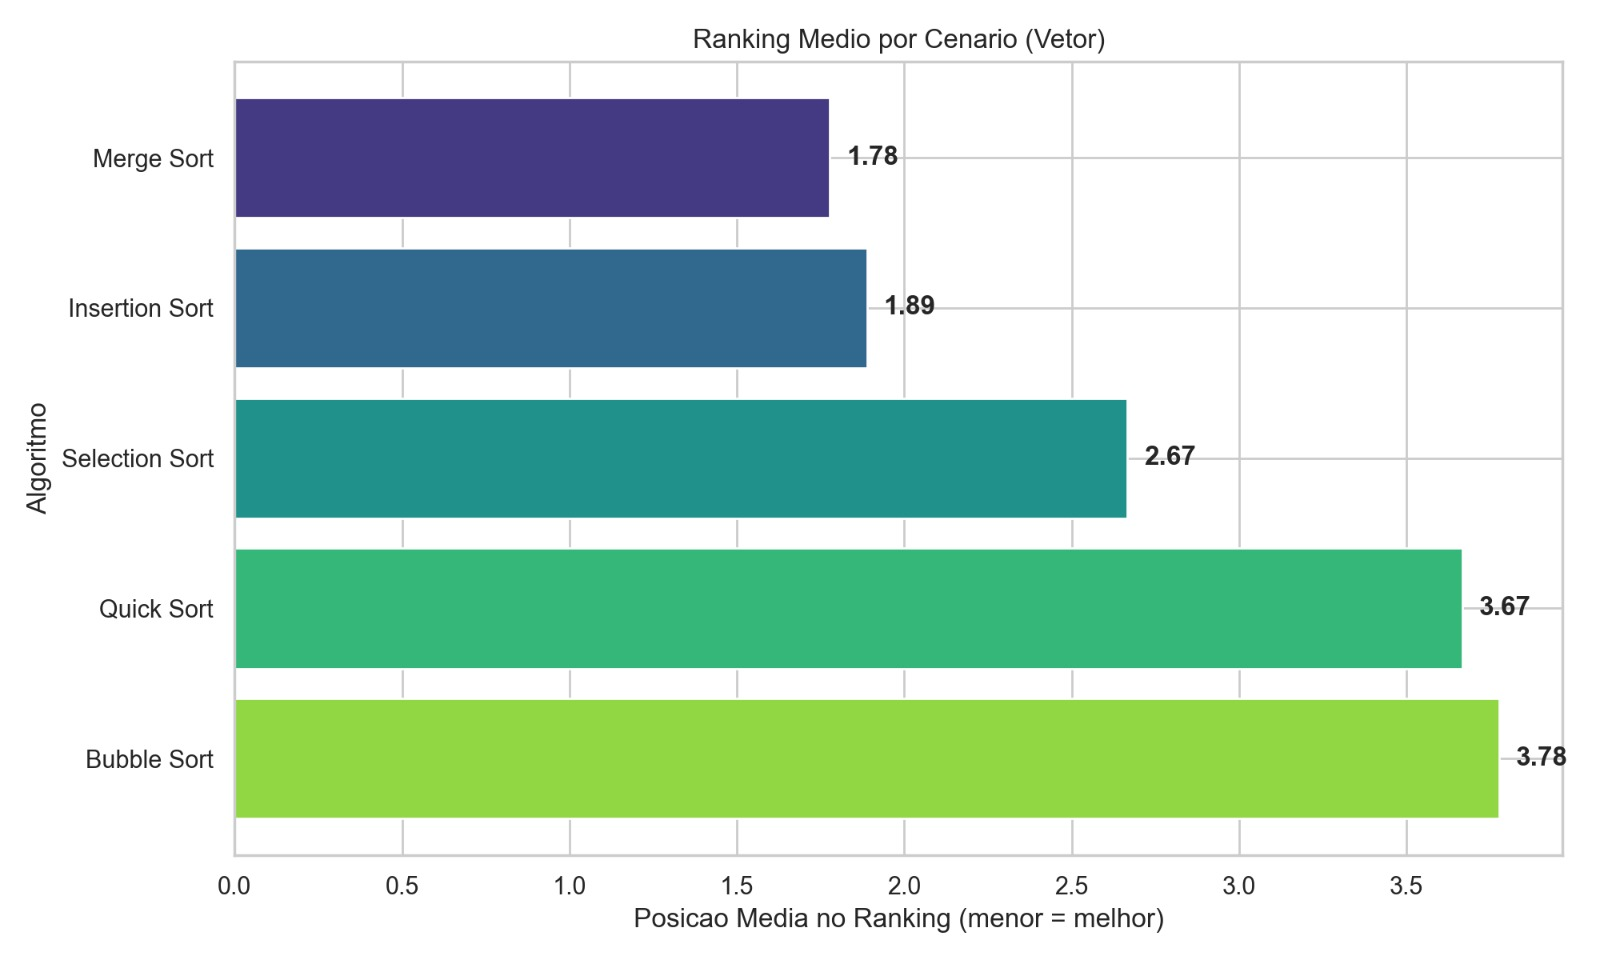
\includegraphics[width=\columnwidth]{grafico_8_heatmap_algoritmo_tamanho.png}
    \caption{Heatmap --- tempo médio (ms) por algoritmo e tamanho no vetor.}
    \label{fig:grafico8}
\end{figure}

\begin{figure}[htbp]
    \centering
    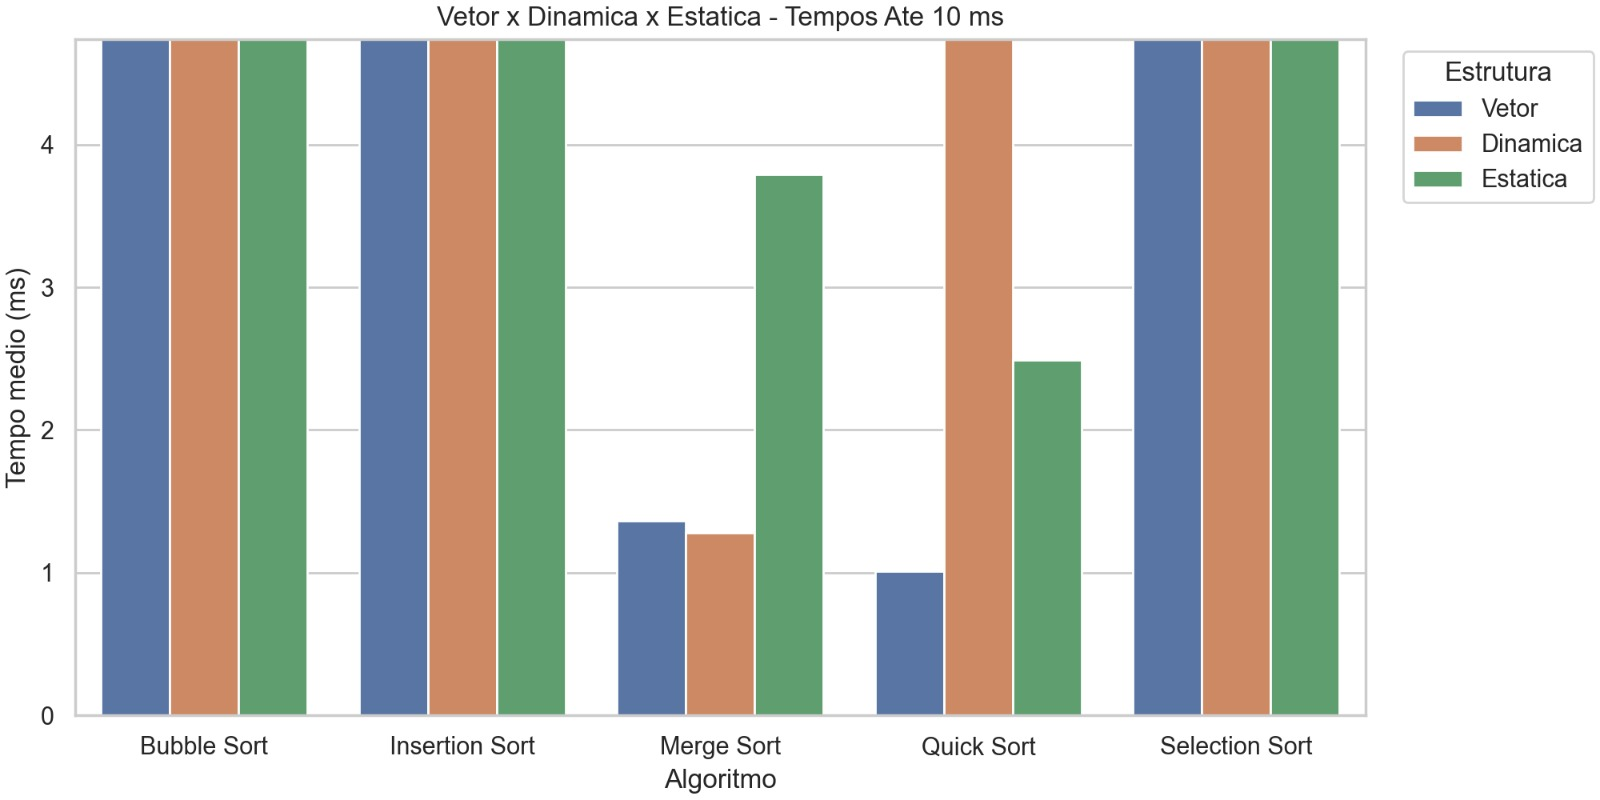
\includegraphics[width=\columnwidth]{grafico_9_ranking_medio.png}
    \caption{Ranking médio por cenário (menor $=$ melhor). Merge Sort e Insertion Sort ocupam as primeiras posições.}
    \label{fig:grafico9}
\end{figure}

O heatmap evidencia que os tempos para $N=100$ e $N=1.000$ são desprezíveis em todos os algoritmos. A diferenciação ocorre em $N=10.000$, onde o Bubble Sort atinge 142\,ms e os algoritmos $O(n \log n)$ ficam abaixo de 2\,ms.

O ranking médio (Figura~\ref{fig:grafico9}) posiciona o Merge Sort em primeiro lugar (1,78) e o Insertion Sort em segundo (1,89), refletindo a adaptatividade deste último para casos ordenados. O Bubble Sort ocupa a última posição (3,78).

\subsection{Síntese dos Resultados}

A Tabela~\ref{tab:resultados} sintetiza os tempos médios para $N=10.000$ com entrada aleatória nas três estruturas.

\begin{table}[htbp]
\centering
\caption{Tempo médio (ms) para $N=10.000$, entrada aleatória}
\label{tab:resultados}
\renewcommand{\arraystretch}{1.2}
\begin{tabular}{lccc}
\toprule
\textbf{Algoritmo} & \textbf{Vetor} & \textbf{Dinâmica} & \textbf{Estática} \\
\midrule
Bubble Sort    & 142,05 & 234,55 & 314,27 \\
Selection Sort &  54,85 & 158,12 & 186,32 \\
Insertion Sort &  40,14 & 125,79 & 152,50 \\
Quick Sort     &   1,01 & 128,97 &   2,49 \\
Merge Sort     &   1,36 &   1,28 &   3,79 \\
\bottomrule
\end{tabular}
\end{table}

% ============================================================
\section{Discussão}
% ============================================================

Os resultados experimentais confirmam, em sua maioria, as previsões da análise teórica de complexidade. Os algoritmos $O(n^2)$ --- Bubble Sort, Selection Sort e Insertion Sort --- apresentaram crescimento quadrático do tempo com o aumento de $N$, enquanto Merge Sort e Quick Sort mantiveram crescimento $O(n \log n)$ para dados aleatórios.

\textbf{Validação da análise teórica.} O Merge Sort demonstrou tempo consistente em todos os cenários, variando de 0,50\,ms (invertido) a 1,36\,ms (aleatório) para $N=10.000$ no vetor. Essa estabilidade é coerente com sua complexidade $O(n \log n)$ invariante. O Quick Sort, por outro lado, confirmou sua vulnerabilidade ao pior caso: para dados ordenados no vetor, atingiu 138,91\,ms --- mais de $137\times$ o tempo no caso aleatório --- comportamento previsto pela análise $O(n^2)$ quando o pivô é extremo.

\textbf{O paradoxo do Insertion Sort.} Um resultado notável é o desempenho do Insertion Sort na lista dinâmica com dados inversamente ordenados: apenas 0,04\,ms. Isso ocorre porque, na implementação para lista dinâmica, a travessia na direção oposta à inserção faz com que o caso ``invertido'' se torne efetivamente o melhor caso, pois cada elemento já se encontra na posição correta da porção ordenada.

\textbf{Impacto das estruturas.} A estrutura de dados influenciou significativamente o desempenho. O vetor apresentou os melhores tempos devido à localidade de cache, enquanto a lista estática foi consistentemente a mais lenta, apesar de seus dados serem contíguos, devido ao custo da navegação por índices e aos padrões de acesso não sequenciais. O Quick Sort foi particularmente afetado na lista dinâmica para entradas ordenadas/invertidas, atingindo mais de 600\,ms --- consequência do acesso sequencial obrigatório para a operação de particionamento em listas encadeadas.

\textbf{Limitações.} O experimento utiliza pivô fixo (último elemento) no Quick Sort, o que provoca degradação severa em dados ordenados e invertidos. Estratégias como mediana-de-três ou pivô aleatório poderiam mitigar este efeito. Além disso, a medição baseada em \texttt{clock()} possui resolução limitada, o que explica leituras de 0\,ms para tamanhos pequenos.

% ============================================================
\section{Conclusão}
% ============================================================

Este trabalho realizou uma análise comparativa abrangente de cinco algoritmos de ordenação em três estruturas de dados, totalizando 135 cenários experimentais (5 algoritmos $\times$ 3 estruturas $\times$ 3 tamanhos $\times$ 3 tipos de entrada), com 100 execuções cada.

Os principais achados são:

\begin{enumerate}
    \item O \textbf{Merge Sort} é o algoritmo mais adequado para a aplicação de ranking de alunos, oferecendo desempenho $O(n \log n)$ garantido, estabilidade e tempos consistentes independentes do padrão de entrada.
    \item A \textbf{estrutura de dados impacta significativamente} o desempenho: o vetor convencional é superior para algoritmos baseados em acesso por índice, enquanto as listas encadeadas introduzem overhead relevante, especialmente para algoritmos $O(n^2)$.
    \item Algoritmos adaptativos como Insertion Sort podem superar algoritmos assintoticamente superiores em cenários favoráveis específicos, mas não oferecem garantias gerais.
    \item O Quick Sort, embora veloz para dados aleatórios, é inadequado para cenários com dados ordenados ou quase ordenados quando utilizada a estratégia de pivô fixa.
\end{enumerate}

Como trabalhos futuros, sugere-se: (i) implementar variantes do Quick Sort com pivô aleatório ou mediana-de-três; (ii) avaliar o impacto de volumes maiores ($N \geq 100.000$); (iii) medir o número de comparações e trocas para complementar a análise temporal; e (iv) comparar com algoritmos híbridos como Introsort e Timsort.

\begin{thebibliography}{9}

\bibitem{cormen}
T.~H. Cormen, C.~E. Leiserson, R.~L. Rivest e C.~Stein, \textit{Algoritmos: Teoria e Prática}, 3ª~ed. Rio de Janeiro: Elsevier, 2012.

\bibitem{sedgewick}
R.~Sedgewick e K.~Wayne, \textit{Algorithms}, 4ª~ed. Boston: Addison-Wesley, 2011.

\bibitem{knuth}
D.~E. Knuth, \textit{The Art of Computer Programming, Vol. 3: Sorting and Searching}, 2ª~ed. Boston: Addison-Wesley, 1998.

\bibitem{ziviani}
N.~Ziviani, \textit{Projeto de Algoritmos com Implementações em C e Pascal}, 3ª~ed. São Paulo: Cengage Learning, 2010.

\end{thebibliography}

\end{document}